\chapter{Word2Vec}

El modelo \textit{word2vec} es una técnica para el procesamiento del lenguaje natural publicada en 2013 (\cite{word2vec:1}, \cite{word2vec:2}).
El algoritmo usa un modelo con una red neuronal para aprender asociaciones entre las palabras de un conjunto de texto. Una vez que el modelo ha
sido entrenado, es posible detectar sinónimos de palabras o incluso sugerir palabras en oraciones incompletas.

Como su nombre indica, \textit{word2vec} representa cada palabra mediante un vector. Estos vectores se escogen de forma que palabras semánticamente similares
estén relativamente cerca entre ellas. Para medir esta cercanía, se usa la similitud coseno:

\begin{definition}
  Dados dos vectores $a,b\in\mathbb{R}$, $n\in\mathbb{N}$, se define la similitud coseno como:
  \[
    S_c(a,b)=\cos\theta = \frac{a\cdot b}{\norm{a}\norm{b}} \in [-1, 1]
  \]
donde $\theta\in[-\pi,\pi]$ es el ángulo entre los vectores $a$ y $b$.
\end{definition}

Es importante notar que la similitud coseno no es una función de medida, ya que no cumple la desigualdad de Schwarz (o desigualdad triangular). El resultado
de esta función indica el nivel de similitud semántica entre las palabras representadas por esos vectores.

A continuación, se presenta cómo se van a obtener esos vectores, y posteriormente, cómo tratar esos vectores para obtener información sobre las palabras. Para
ello, se presentan dos variantes del modelo.

\section{Coninuous Bad-of-Word Model}

\subsection{Contexto de una sola palabra}

Primero se va a desarrollar el modelo \textit{bolsa de palabras continuas} (o CBOW, por sus siglas en inglés) considerando que el contexto está formado por una única palabra.
Esto será útil para establecer la notación para el resto del trabajo. Que haya una única palabra por contexto implica que el modelo precidirá también una única palabra objetivo.
Por lo tanto, se está presentando un modelo \textit{bigram} (es decir, que usa dos palabras).

\begin{figure}[H]
  \centering
  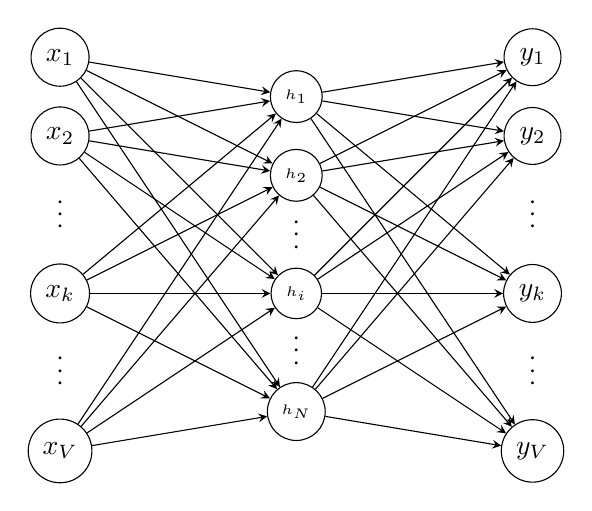
\begin{tikzpicture}[
          roundnode/.style={circle, draw=black, minimum size=4mm},
      ]

      \node[roundnode]   at (1,4)   (inputV)  {$x_V$};
      \node[roundnode]   at (1,6)   (inputK)  {$x_k$};
      \node[roundnode]   at (1,8)   (input2)  {$x_2$};
      \node[roundnode]   at (1,9)   (input1)  {$x_1$};

      \path (input2) -- (inputK) node [black, midway, sloped] {$\dots$};
      \path (inputK) -- (inputV) node [black, midway, sloped] {$\dots$};

      \node[roundnode]   at (4,4.5)   (hiddenN)  {\tiny $h_N$};
      \node[roundnode]   at (4,6)     (hiddenI)  {\tiny $h_i$};
      \node[roundnode]   at (4,7.5)   (hidden2)  {\tiny $h_2$};
      \node[roundnode]   at (4,8.5)   (hidden1)  {\tiny $h_1$};

      \path (hidden2) -- (hiddenI) node [black, midway, sloped] {$\dots$};
      \path (hiddenI) -- (hiddenN) node [black, midway, sloped] {$\dots$};

      \draw[-stealth] (input1) -- (hidden1);
      \draw[-stealth] (input1) -- (hidden2);
      \draw[-stealth] (input1) -- (hiddenI);
      \draw[-stealth] (input1) -- (hiddenN);
      \draw[-stealth] (input2) -- (hidden1);
      \draw[-stealth] (input2) -- (hidden2);
      \draw[-stealth] (input2) -- (hiddenI);
      \draw[-stealth] (input2) -- (hiddenN);
      \draw[-stealth] (inputK) -- (hidden1);
      \draw[-stealth] (inputK) -- (hidden2);
      \draw[-stealth] (inputK) -- (hiddenI);
      \draw[-stealth] (inputK) -- (hiddenN);
      \draw[-stealth] (inputV) -- (hidden1);
      \draw[-stealth] (inputV) -- (hidden2);
      \draw[-stealth] (inputV) -- (hiddenI);
      \draw[-stealth] (inputV) -- (hiddenN);


      \node[roundnode]   at (7,4)   (outputV)  {$y_V$};
      \node[roundnode]   at (7,6)   (outputI)  {$y_k$};
      \node[roundnode]   at (7,8)   (output2)  {$y_2$};
      \node[roundnode]   at (7,9)   (output1)  {$y_1$};

      \path (output2) -- (outputI) node [black, midway, sloped] {$\dots$};
      \path (outputI) -- (outputV) node [black, midway, sloped] {$\dots$};

      \draw[-stealth] (hidden1) -- (output1);
      \draw[-stealth] (hidden1) -- (output2);
      \draw[-stealth] (hidden1) -- (outputI);
      \draw[-stealth] (hidden1) -- (outputV);
      \draw[-stealth] (hidden2) -- (output1);
      \draw[-stealth] (hidden2) -- (output2);
      \draw[-stealth] (hidden2) -- (outputI);
      \draw[-stealth] (hidden2) -- (outputV);
      \draw[-stealth] (hiddenI) -- (output1);
      \draw[-stealth] (hiddenI) -- (output2);
      \draw[-stealth] (hiddenI) -- (outputI);
      \draw[-stealth] (hiddenI) -- (outputV);
      \draw[-stealth] (hiddenN) -- (output1);
      \draw[-stealth] (hiddenN) -- (output2);
      \draw[-stealth] (hiddenN) -- (outputI);
      \draw[-stealth] (hiddenN) -- (outputV);

  \end{tikzpicture}
  \caption{CBOW con 1 palabra por contexto}
  \label{redneuronal:3}
\end{figure}

En la figura \ref{redneuronal:3}, se muestra la versión simplificada de la red neuronal, donde el tamaño del vocabulario es $V\in\mathbb{N}$ y el tamaño de la capa escondida es $N\in\mathbb{N}$.
Las unidades entre capas adyacentes están conectadas totalmente a todas las unidades de la otra capa y viceversa. Como input de la red se usa un \textit{one-hot encoded vector},
que simplemente es un vector de tamaño $V$ donde cada posición representa una palabra. Es decir, si arbitrariamente, se deduce que la palabra 'coche` se va a representar en la $k-$ésima
posición, entonces el vector $(0, \dots, 1, \dots, 0)$ con un 1 en la $k-$ésima posición, sería la representación de la palabra coche.

Los pesos entra la capa de entrada y la de salida pueden ser representados por una matriz $W\in\mathbb{R}^{V\times N}$, donde cada fila de $W$ es la representación
vectorial $N-$dimensional de la palabra $w$ asociada en la capa de entrada. Las filas de esta matriz son la represención vectorial $N$-dimensional, $v_{w_I}$ (donde $I\in\{1, \ldots, V\}$),
de la palabra $w$ de entrada (representada por $x$).

Dado entonces un contexto con una única palabra, $w_I$, se tiene su representación como vector de entrada $x\in\mathbb{R}^V$, de forma que $x_k=1$ con $x_{k'}=0$ si $k'\neq k$. A partir de
$W$ y $x$, se puede obtener el vector $N$-dimensional de la capa intermedia, de la siguiente forma:
\begin{equation}\label{eq:h}
  h=W^Tx=W^T_{k, \cdot}=v^T_{w_I}
\end{equation}
donde es importante resaltar que esta operación no es más que copiar la fila $k$-ésima de $W$ en $h$. Esa fila fue denotada en el párrafo anterior por $v_{w_I}$.
Esto significa que la función de activación de la capa escondida es simplemente linear, es decir, pasa directamente la suma ponderada de sus inputs a la siguiente capa.

De forma similar, se puede operar de la capa escondida a la capa de salida, donde se tiene una matriz de pesos diferente, $W'\in\mathbb{R}^{N\times V}$. En esta matriz, la representación
de cada palabra viene dada por cada una de sus columnas, es decir, la representación de la palabra $w_j$ en $W'$, es la columna $j$-ésima de $W'$ y es representada por $v'_{v_{w_j}}$. Con
esta notación, se puede calcular ahora un escalar (antes se ha calculado un vector) $u_j$ para cada una de las palabras del vocabulario:
\begin{equation}\label{eq:uj}
  u_j = v_{w_j}^{'T}h
\end{equation}
Finalmente, se puede usar \textit{softmax}, un modelo de clasificación lineal logarítmico, para obtener una distribución de las palabras (que es una distribución multinomial):
\begin{equation}\label{eq:yj}
p(w_j|w_I) = \frac{\exp(u_j)}{\sum_{j'=1}^V\exp(u_{j'})} =: y_j
\end{equation}
donde $y_j$ es el valor de la $j$-ésima neurona de la capa de salida. Una vez se tiene esta expresión, se pueden sustituir los valores de $u_j$ y $u_j'$ por los obtenidos
en párrafos anteriors, llegando a la siguiente fórmula:
\begin{equation}\label{eq:4}
  p(w_j|w_I) = \frac{\exp(w^{'T}_{w_j}v_{w_I})}{\sum_{j'=1}^V\exp(v^{'T}_{w_{j'}}v_{w_I})}
\end{equation}

Como clarificación, es importante recordar que $v_w$ y $v'_w$, son representaciones distintas de la palabra $w$:
\begin{itemize}
  \item $v_w$ proviene de las filas de la matriz $W$. Normalmente es denominado el vector de entrada.
  \item $v'_w$ proviene de las columnas de la matriz $W'$. Normalmente es denominado el vector de salida.
\end{itemize}

\subsubsection*{Actualización de pesos de capa escondida a capa de salida}

A continuación se presenta el desarrollo para la ecuación de actualización de pesos de este modelo. El objetivo de
entrenamiento (para una muestra de entrenamiento) es maximizar \ref*{eq:4}, que no es más que la probabilidad condicionada
de observar una palabra $w_O$ (denotando a su índice en la capa de salida por $j^*$), dada la palabra del contexto $w_I$:
\begin{equation}
  \begin{split}
  \max p(w_O|w_I) & = \max y_{j^*}\\
         & =\max \log(y_{j^*})\\
         & = u_{j^*} - \log \sum_{j'=1}^V\exp(u_{j'}) := -E \\
  \end{split}
\end{equation}
de donde se deduce que $E=-\log p(w_O|w_I)$ es la función de pérdida del modelo (porque es la función que se quiere minimizar).

Ahora es posible deducir la equación de actualización de pesos entre la capa escondida y la de salida. Para ello, se calcula
la derivada de $E$ respecto al escalar $u_j$, que se definió anteriormente para cada palabra:
\begin{equation}
  \begin{split}
  \frac{\partial E}{\partial u_j} & = \left(-u_{j*}+ \log\sum_{j'=1}^V\exp(u_{j'})\right)\frac{\partial}{\partial u_j} \\
  \end{split}
\end{equation}
Para el desarrollo de esa expresión, es importante resaltar que $j^*\neq j$, por lo que la expresión resultante queda mucho
más simple:
\begin{equation}
  \frac{\partial E}{\partial u_j} = y_j - t_j, \;\; \forall j \in \{1, \cdots, V\}
\end{equation}
donde $y_j$ fue definido en \ref*{eq:yj} y $t_j$ es definido, por simplicidad, como:
\[ t_j = \begin{cases}
  1 & j = j^* \\
  0 & j \neq j^*
\end{cases}
\]
Es importante notar que lo que se acaba de calcular no es más ni menos que la componente $j$-ésima del error de predicción de la capa de salida, por lo tanto,
se puede notar como:
\begin{equation}\label{eq:ej}
  \frac{\partial E}{\partial u_j} = y_j - t_j := e_j, \;\; \forall j \in \{1, \cdots, V\}
\end{equation}
Ahora es necesario calcular el gradiente en los pesos entre la capa escondida y de salida (que fueron denotados por $W'=\{w'_{ij}\}$). Para ello,
basta con derivar la misma expresión pero respecto de $w'_{ij}$:
\begin{equation}
  \frac{\partial E}{\partial w'_{ij}} = \frac{\partial E}{\partial u_j} \frac{\partial u_j}{\partial w'_{ij}} = e_j h_i
\end{equation}
Por lo tanto, ya se puede aplicar la técnica de descenso de gradiente porque se ha obtenido la ecuación de actualización de pesos para cada uno de los valores de $W'$:
\[
  w_{ij}^(nuevo) = w_{ij}^{'(viejo)} - \eta e_jh_i
\]
En lugar de escalar a escalar, esa expresión también se puede escribir usando la representación vectorial de la palabra $w$ en $W'$, es decir, $v'_{w_j}$:
\[
  v_{w_j}^{'(nuevo)}=v_{w_j}^{'(viejo)} - \eta e_j h, \;\;\; j \in \{1, \cdots, V\}
\]
donde $\eta > 0$ es el ratio de aprendizaje.

Es importante resaltar que esta ecuación implica que es necesario recorrer cada posible palabra en el vocabulario, comprobar su probalidad de la capa de salida, $y_j$, y
compararlo con su valor esperado, $t_j$ (que solo puede ser 0 o 1). Si se da $y_j > t_j $ (caso de sobreestimación) entonces se resta una proporción de $h$ (se recuerda que
$h=v_{w_I}$) a $v'_{w_j}$. Si se tiene el caso contrario, entonces se realiza la operación contraria. En ambos casos, $v'_{w_O}$ es cada vez más cercano a $v_{w_I}$ (en
este caso la \textit{cercanía} usa el producto escalar y no la distancia euclídea usual).

\subsubsection*{Actualización de pesos de capa de entrada a capa escondida}

Una vez obtenida la ecuación para actualizar los pesos de la capa escondida a la de salida, se pueden usar usar esos mismos cálculos para calcular
la ecuación de actualización de la capa anterior (\textit{back-propagation}), es decir, de la capa de entrada a la de salida.

Para obtener esa ecuación, es necesario minimizar una vez más la función de error $E$, pero esta vez con respecto a $h_i$:
\begin{equation}
  \frac{\partial E}{\partial h_i} = \sum_{j=1}^V\frac{\partial E}{\partial u_j} \frac{\partial u_j}{\partial h_i} = \sum_{j=1}^Ve_j w'_{ij} := EH_i, \;\; \forall i \in \{1, \cdots, N\}
\end{equation}
donde $h_i$ es la $i$-ésiima componente de la capa escondida, $u_j$ se definió en \ref*{eq:uj} y $e_j$ se definió en \ref*{eq:ej} como el error de predicción
de la $j$-ésima unidad de la capa de salidad. A partir de $EH_i$, se puede definir un vector de dimensión $N$, en el que cada componente es la suma de los vectores
de salida de todas las palabras, promediados por el error de predicción.

El siguiente paso sería calcular la derivada de $E$ con respecto de $W$. Primero, se recuerda que la capa escondida simplemente es una función linear de los valores de la capa de entrada. Expandiendo
la notación vectorial de \ref*{eq:h}, se obtiene:
\begin{equation}
  h_i=\sum_{k=1}^Vx_kw_k{ki}
\end{equation}
Usando esa expresión se puede derivar $E$ con respecto a cada elemento de $W$, obteniendo:
\begin{equation}
  \frac{\partial E}{\partial w_{ki}} = \frac{\partial E}{\partial h_i} \frac{\partial h_i}{\partial w_{ki}} = EH_i x_k
\end{equation}
Con ese resultado, se puede expresar $\frac{\partial E}{\partial W}=xEH^T$. Como solo un componente de $x$ es distinto de cero (se recuerda que se están usando \textit{one-hot encoded vectors}), solo
una fila de $\frac{\partial E}{\partial W}$ es distinta de cero, y su valor es $EH^T$, un vector $N$-dimensional.  Finalmente, se puede obtener la ecuación de actualización de $W$:
\begin{equation}
  v_{w_I}^{(nuevo)} - v_{w_I}^{(antiguo)} - \eta EH^T
\end{equation}
donde $v_{w_I}$ es una fila de $W$, la representación del vector de entrada (la única palabra del contexto). Como consecuecnia de que solo una fila de $\frac{\partial E}{\partial W}$ sea distinta de 0,
es que todas las otras filas de $W$ permanecerán sin cambiar después de esta iteración.

De igual forma que en el apartado anterior, si la probabilidad de una palabra $w_j$ es sobreestimada ($y_j>t_j$), entonces el vector de entrada de la palabra del contexto $w_I$ tenderá a alejarse del vector de salida
de $w_j$. Lo contrario es cierto, si la probabilidad es subestimada. Por lo tanto, el movimiento del vector de entrada de $w_I$ es determinado por el error de predicción de todos los vectores en el vocabulario. Cuanto más
grande sea el error de predicción, más significativo será el cambio en el vector de entrada de la palabra del contexto.

Conforme se actualizan los parámetros del modelo de forma iterativa, los efectos de cada iteración se van a ir acumulando. Se puede imaginar que el vector de salida de una palabra $w$ es `arrastrado' de un lado hacia otro
por los vectores de entrada de los vecinos de $w$.
\subsection{Contexto de múltiples palabras}

\begin{figure}[H]
  \centering
  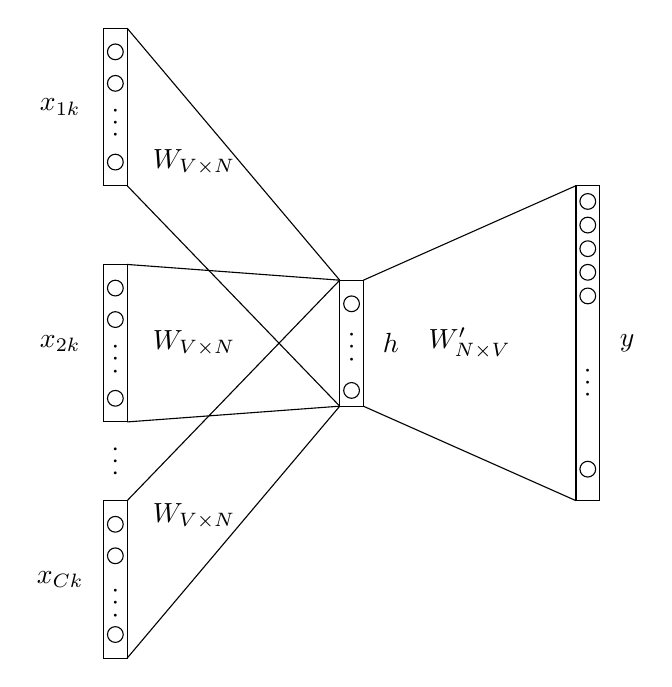
\begin{tikzpicture}[
          roundnode/.style={circle, draw=black, minimum size=4mm},
      ]

      \node[rectangle, draw, minimum width = 0.3cm, minimum height = 2cm] (xck) at (0.5,0) {};
      \node[] at (-0.2,0) {$x_{Ck}$};
      \draw[] (0.5, 0.7) circle (0.1cm);
      \draw[] (0.5, 0.3) circle (0.1cm);
      \draw[] (0.5, -0.7) circle (0.1cm);
      \path (0.5, -0.9) -- (0.5, 0.3) node [black, midway, sloped] {$\dots$};

      \node[rectangle, draw, minimum width = 0.3cm, minimum height = 2cm] (xdk) at (0.5,3) {};
      \node[] at (-0.2,3) {$x_{2k}$};
      \draw[] (0.5, 3.7) circle (0.1cm);
      \draw[] (0.5, 3.3) circle (0.1cm);
      \draw[] (0.5, 2.3) circle (0.1cm);
      \path (0.5, 2.3) -- (0.5, 3.3) node [black, midway, sloped] {$\dots$};

      \node[rectangle, draw, minimum width = 0.3cm, minimum height = 2cm] (xuk) at (0.5,6) {};
      \node[] at (-0.2,6) {$x_{1k}$};
      \draw[] (0.5, 6.7) circle (0.1cm);
      \draw[] (0.5, 6.3) circle (0.1cm);
      \draw[] (0.5, 5.3) circle (0.1cm);
      \path (0.5, 5.3) -- (0.5, 6.3) node [black, midway, sloped] {$\dots$};

      \path (xdk) -- (xck) node [black, midway, sloped] {$\dots$};

     % ========= hidden layer


      \node[rectangle, draw, minimum width = 0.3cm, minimum height = 1.6cm] (xdk) at (3.5,3) {};
      \node[] at (4,3) {$h$};
      \draw[] (3.5, 3.5) circle (0.1cm);
      \draw[] (3.5, 2.4) circle (0.1cm);
      \path (3.5, 2.4) -- (3.5, 3.5) node [black, midway, sloped] {$\dots$};

     % ========= connections input->hidden layer

     \draw[] (0.65,1) -- (3.35,3.8);
     \draw[] (0.65,4) -- (3.35,3.8);
     \draw[] (0.65,7) -- (3.35,3.8);

     \draw[] (0.65,-1) -- (3.35,2.2);
     \draw[] (0.65,2) -- (3.35,2.2);
     \draw[] (0.65,5) -- (3.35,2.2);

     \node[] at (1.5,0.8) {$W_{V\times N}$};
     \node[] at (1.5,3) {$W_{V\times N}$};
     \node[] at (1.5,5.3) {$W_{V\times N}$};


     % ========= output layer

     \node[rectangle, draw, minimum width = 0.3cm, minimum height = 4cm] (xdk) at (6.5,3) {};
     \node[] at (7,3) {$y$};
     \draw[] (6.5, 4.8) circle (0.1cm);
     \draw[] (6.5, 4.5) circle (0.1cm);
     \draw[] (6.5, 4.2) circle (0.1cm);
     \draw[] (6.5, 3.9) circle (0.1cm);
     \draw[] (6.5, 3.6) circle (0.1cm);
     \draw[] (6.5, 1.4) circle (0.1cm);
     \path (6.5, 1.4) -- (6.5, 3.6) node [black, midway, sloped] {$\dots$};


     % ========= connections hidden->output layer

     \draw[] (3.65,3.8) -- (6.35, 5);
     \draw[] (3.65,2.2) -- (6.35, 1);

     \node[] at (5,3) {$W'_{N\times V}$};

  \end{tikzpicture}
  \caption{CBOW con C palabras por contexto}
  \label{redneuronal:4}
\end{figure}
